\documentclass[10pt,a4paper]{article}
\usepackage[top=0in, bottom=0.5in,margin=1in, includefoot]{geometry}
\usepackage[utf8]{inputenc}
\usepackage[T1]{fontenc}

\title{Numerical analysis - Exercise 1}
\author{}
\date{}

\usepackage{graphicx}
\usepackage[export]{adjustbox}
\usepackage{ulem}
\setlength\parindent{0pt}
\usepackage{amsmath}
\usepackage{wrapfig}
\usepackage{subcaption}
\usepackage{lineno}
\usepackage{layout}
\usepackage{alltt}
\usepackage[section]{placeins}

\setlength{\voffset}{-0.4in}
\textheight = 735pt
\begin{document}
\vspace{-20mm}
\title{\textbf{EE2-08C Numerical Analysis} \\ Group 9\vspace{-17mm}}
\maketitle
\section{Exercise 2 - Error Analysis for RL Circuit}\vspace{-1mm}

\begin{subsection}{Introduction}
In Exercise 1, three numerical methods(Heun,Midpoint and Ralston) were used to estimate the value of functions for different inputs. However,these numerical methods have errors and do not give the exact solutions to the ODE. Therefore, in Exercise 2, the exact solutions to the ODEs will be obtained using MATLAB. These solutions will then be compared with those obtained using the numerical methods (in Exercise 1) to estimate the errors associated with the numerical methods. 
\end{subsection}
\section{Exact Value}
For this RL circuit, a linear first order ODE is used to obtain the exact equation.
\begin{subsection}{Linear first order ODE}

\begin{equation}
\frac{dy}{dx}+p(x)y=Q(x)
\end{equation}

\begin{equation}
y(x)=Ce^{-\int{P(x)dx}}+e^{-\int{P(x)dx}}\int{Q(x)e^{\int{P(x)dx}}dx}
\end{equation}

\end{subsection}

\begin{subsection}{Linear first order ODE for RL circuit}

\begin{equation}
v_L(t)+v_R(t)=V_{in}(t)
\end{equation}
\begin{equation}
L\frac{di_L(t)}{dt}+Ri_L(t)=V_{in}(t)
\end{equation}

\begin{equation}
R=0.5\Omega
L=1.5mH
\end{equation}

Input is given as
\begin{equation}
V_{in}=6cos(\frac{2{\pi}t}{150*{10^{-6}}})
\end{equation}

According to linear first order ODE, we get:

\begin{equation}
1.5*10^{-3}\frac{di_L(t)}{dt}+0.5i_L(t)=6cos(\frac{2{\pi}t}{150*{10^{-6}}})
\end{equation}

\begin{equation}
\frac{di_L(t)}{dt}+\frac{1}{3}*10^3i_L(t)=4*10^3cos(\frac{2{\pi}t}{150*{10^{-6}}})
\end{equation}

\begin{equation}
e^{{\frac{1}{3}*10^3}t}\frac{di_L(t)}{dt}+e^{{\frac{1}{3}*10^3}t}*\frac{1}{3}*10^3i_L(t)=e^{{\frac{1}{3}*10^3}t}*4*10^3cos(\frac{2{\pi}t}{150*{10^{-6}}})
\end{equation}

\begin{equation}
\frac{d(e^{{\frac{1}{3}*10^3}t}i_L(t))}{dt}=e^{{\frac{1}{3}*10^3}t}*4*10^3cos(\frac{2{\pi}t}{150*{10^{-6}}})
\end{equation}

Integrate both sides of the equation:

\begin{equation}
exact=-\frac{12}{1600\pi^2+1}exp(-1000/3t)+\frac{480\pi}{1600\pi^2+1}sin(\frac{40000t\pi}{3})+\frac{1}{1600\pi^2+1}cos(\frac{40000t\pi}{3})
\end{equation}
\end{subsection}
\begin{subsection}{Error Functions} 
Using the same MATLAB scripts in Exercise 1 (heun.m,midpoint.m and ralston.m) the estimated values for the ODEs can be obtained. The result of subtracting these estimated solutions from the exact solutions leads to the error functions. In this section, the error functions will be developed using this technique for the three numerical analysis methods.

\begin{subsection}{Heun's Method}

\begin{figure}[h]
    \centering
    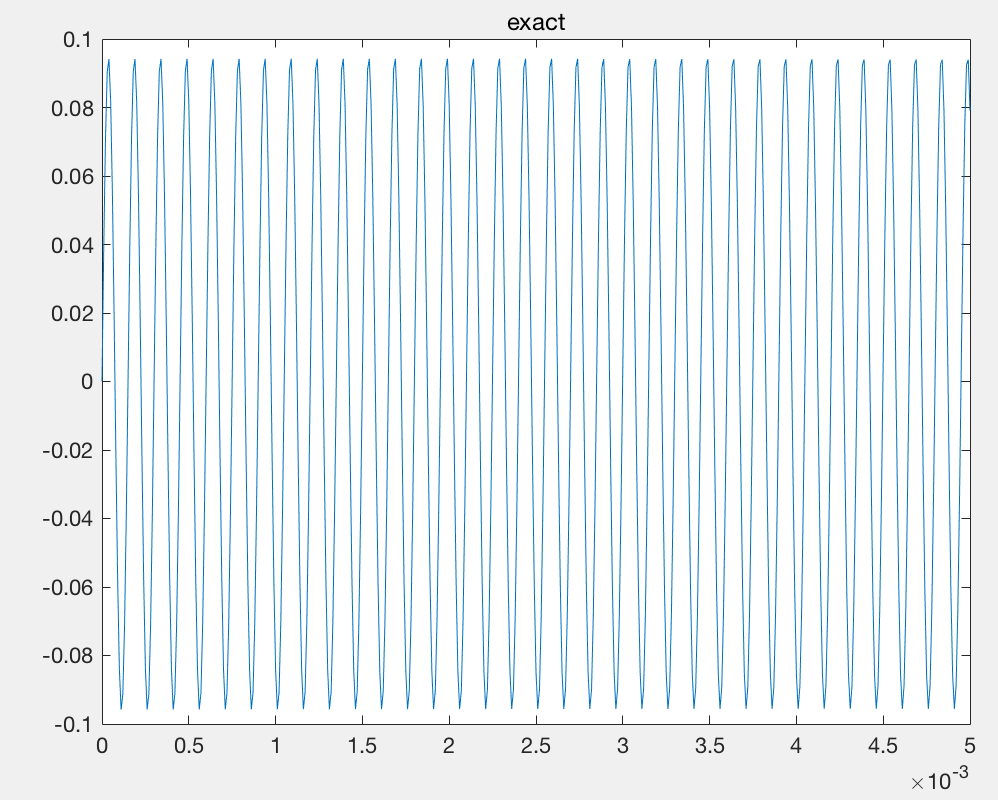
\includegraphics[scale=0.5]{heun_error_exact}
    \caption{Exact Value}
    \label{fig:Exact Value}
\end{figure}

Figure \ref{fig:Exact Value} shows the exact solution to the ODE. Figure \ref{fig:Heun Method} shows the estimated solution using Heun's method. When the estimated solution is subtracted from the exact solution, the resulting function is the error function for Heun's method which is plotted in figure \ref{fig:heun_error}.

\begin{figure}[h]
\begin{subfigure}{.5\textwidth}
  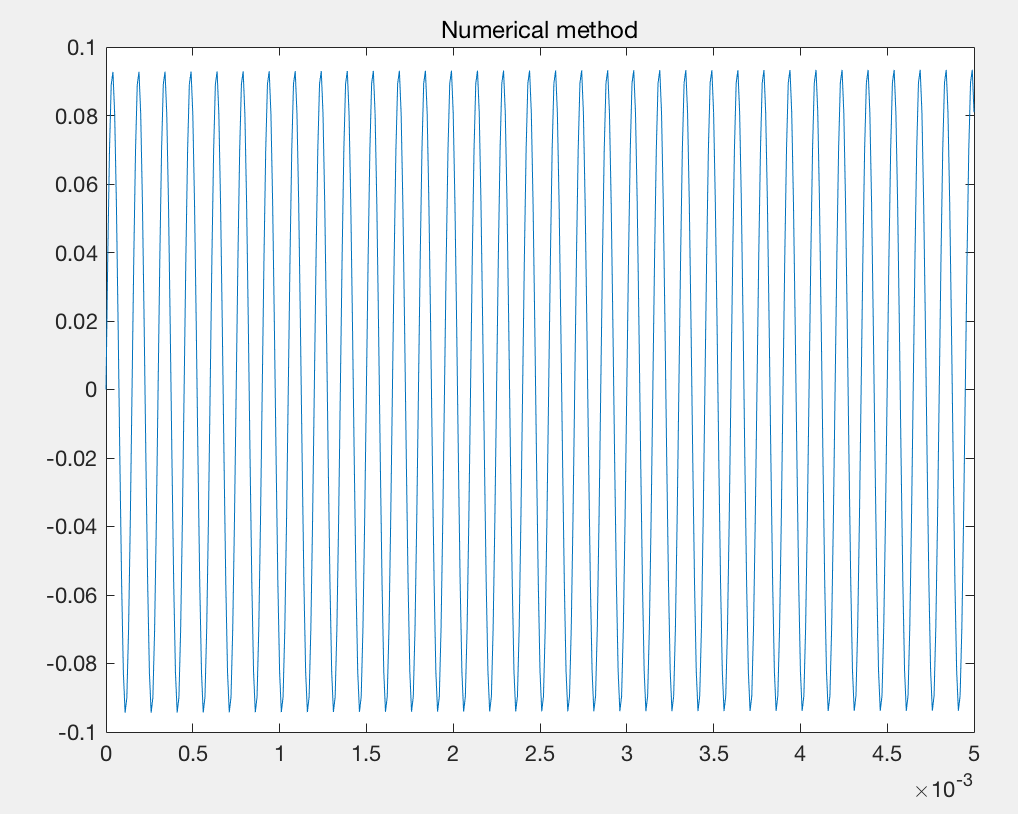
\includegraphics[width=.9\linewidth,height = 5cm
  ]{heun_error_numerical_method}
  \caption[right]{Heun's Method}
  \label{fig:Heun Method}
\end{subfigure}
\begin{subfigure}{.5\textwidth}
  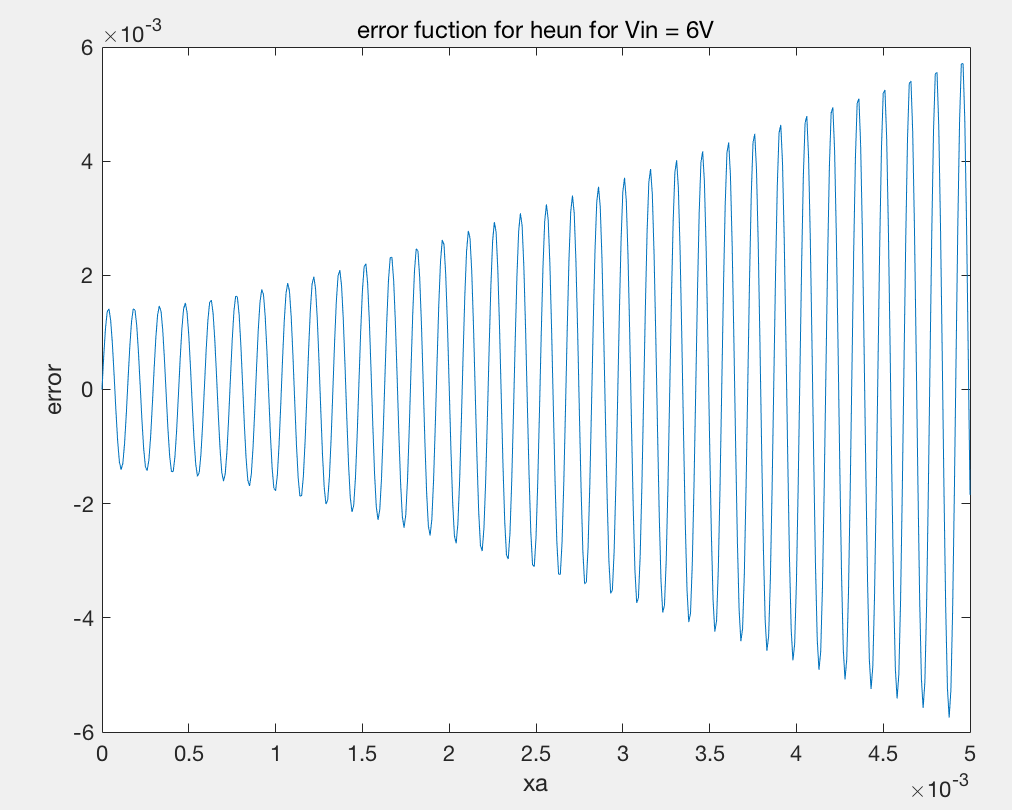
\includegraphics[width=.9\linewidth,height = 5cm]{heun_error}
  \caption{Error function for Heun's Method}
  \label{fig:heun_error}
\end{subfigure}
\caption{Estimated solution and Error Function for Heun's method}
\label{fig:Heun_Error_sub}
\end{figure}



%% Add comments on the error function for Heun's method.

\end{subsection}
\clearpage

\begin{subsection}{Midpoint method}
The same analysis is used to obtain the error function for Midpoint method. The exact solution for the ODE is the same as that for Heun's method (Figure \ref{fig:Exact Value}).  Figure \ref{fig:midpoint_method} shows the estimated solution obtained by using the midpoint method. Similar to Heun's error analysis, when the estimated solution is subtracted from the exact solution, the resulting function is the error function. This error function is plotted in figure \ref{fig:midpoint_error}.

\begin{figure}[h]
\begin{subfigure}{.5\textwidth}
  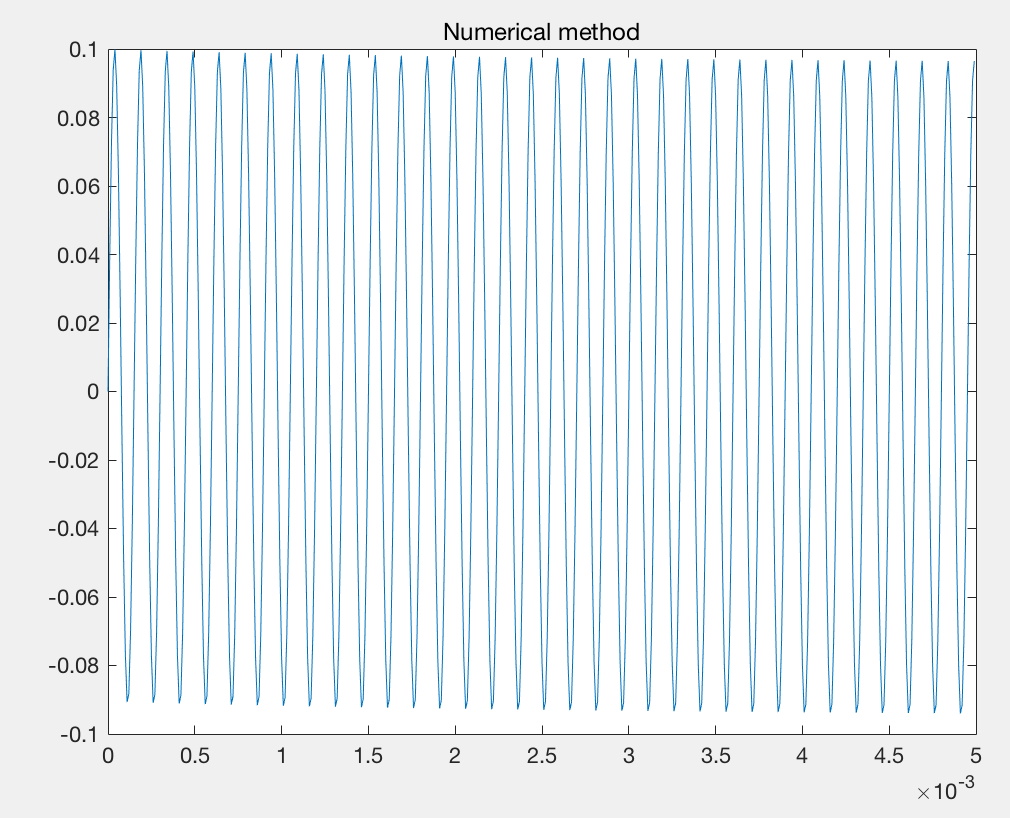
\includegraphics[width=.9\linewidth,height = 5cm
  ]{midpoint_error_numerical_method}
  \caption[right]{Midpoint Method}
  \label{fig:midpoint_method}
\end{subfigure}
\begin{subfigure}{.5\textwidth}
  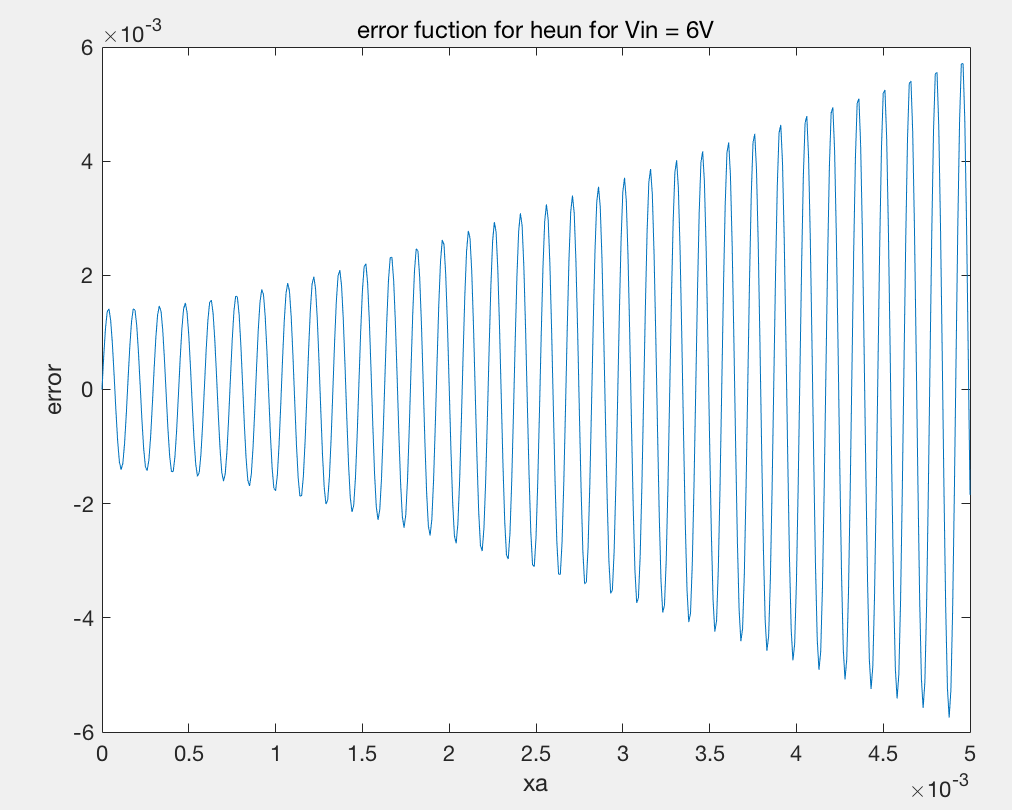
\includegraphics[width=.9\linewidth,height = 5cm]{heun_error}
  \caption{Error function for Midpoint Method}
  \label{fig:midpoint_error}
\end{subfigure}
\caption{Estimated solution and Error Function for Midpoint method}
\label{fig:Method_Error_sub}
\end{figure}

%%Add comments on the error function for Midpoint here

\end{subsection}

\begin{subsection}{Ralston method}
Making use of the same error analysis technique as above(for Heun's and Midpoint methods), the estimated value obtained using the Ralston method is in figure \ref{fig:ralston_method} and the error function is plotted in figure \ref{fig:ralston_error}.

\begin{figure}[h]
\begin{subfigure}{.5\textwidth}
  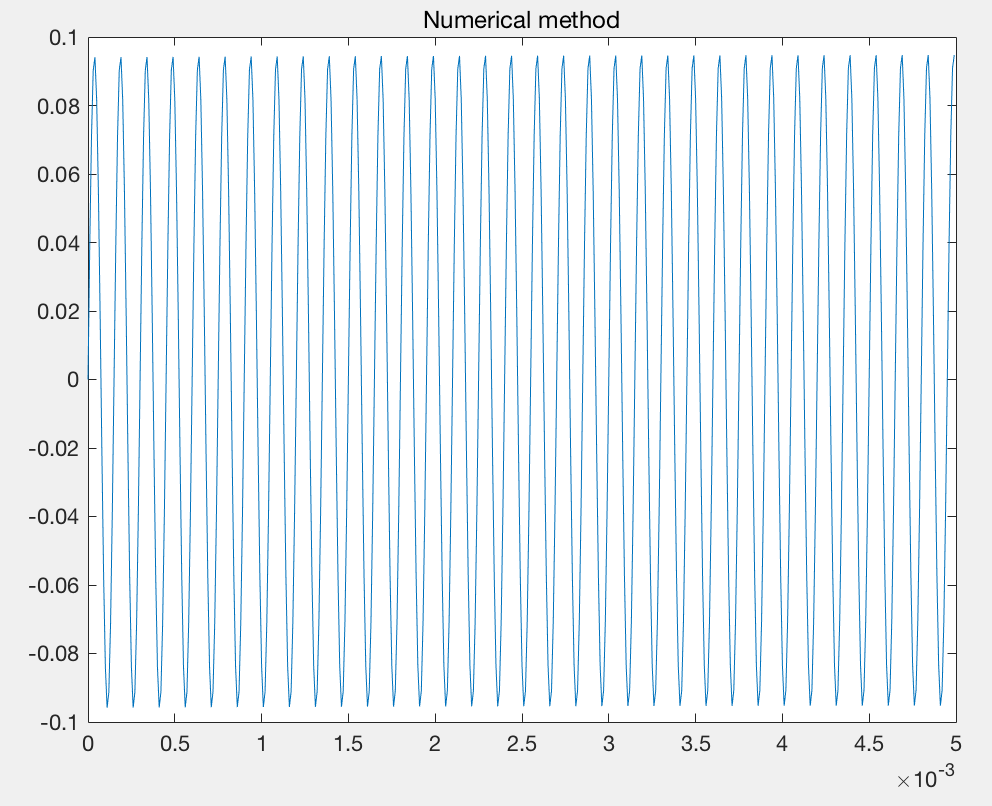
\includegraphics[width=.9\linewidth,height = 5cm
  ]{ralston_error_numerical_method}
  \caption[right]{Ralston Method}
  \label{fig:ralston_method}
\end{subfigure}
\begin{subfigure}{.5\textwidth}
  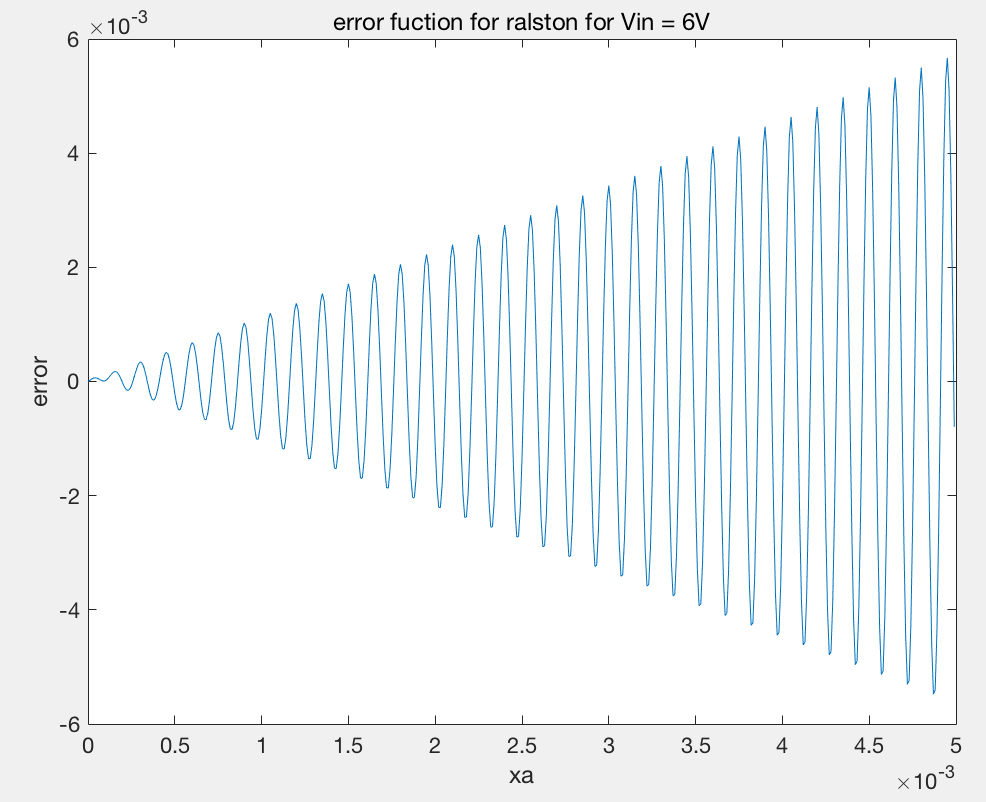
\includegraphics[width=.9\linewidth,height = 5cm]{ralston_error}
  \caption{Error function for Ralston Method}
  \label{fig:ralston_error}
\end{subfigure}
\caption{Estimated solution and Error Function for Ralston method}
\label{fig:Ralston_Error_sub}
\end{figure}


%%Add comments on Ralston error function here
\end{subsection}
\clearpage

\subsection{Comparison}
For Heun's error function, the error increases from
$\underline{+}1.1*10^{-3}$ at 0 to $\underline{+}5.9*10^{-3}$ at $5*10^{-3}$. For the Midpoint error function, the error icreases from [-0.01,0] at 0 to [-0.011,0.01] at $5*10^{-3}$.
Finally, for Ralston's error function the error increases from 0 at 0 to $\underline{+}5.9*10^{-3}$ at $5*10^{-3}$.

Therefore, we can deduce that the Ralston method has the least error in approximating solutions for the linear first order ODE. %%Is this true?

\begin{subsection}{Log-log plot}
\begin{figure}[h]
    \centering
    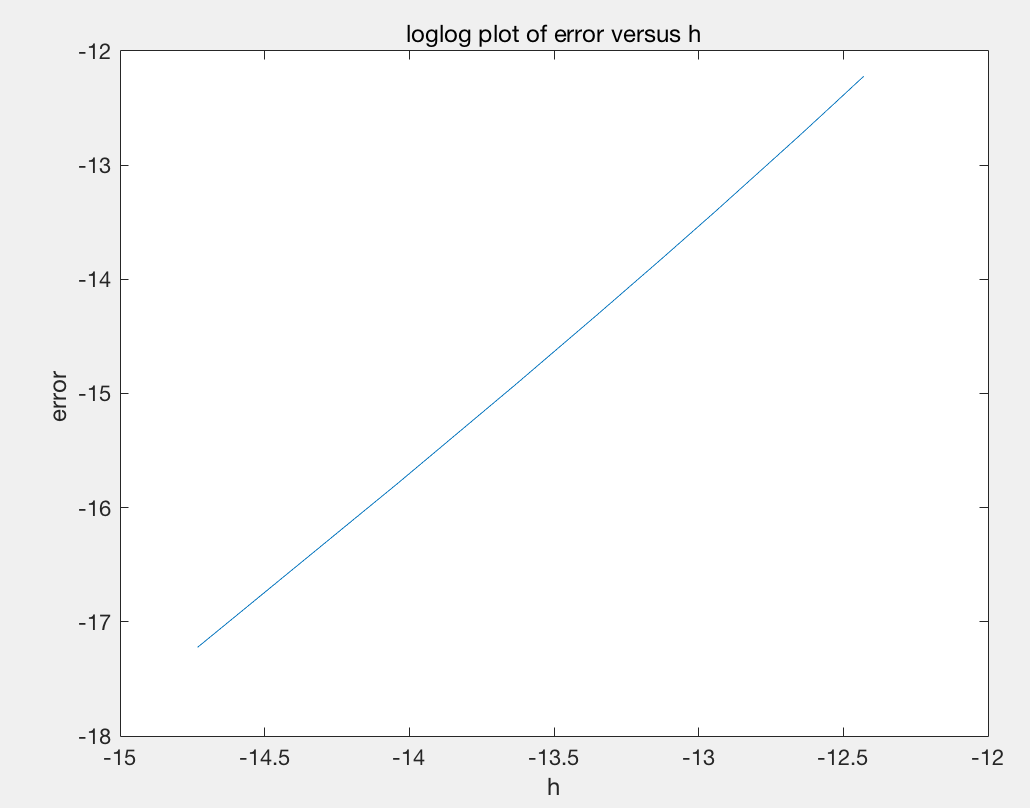
\includegraphics[scale=0.5]{errorloglogfinal1}
    \caption{Log-Log plot for Ralston method}
    \label{fig:heun_error_loglog} %%heun's or ralston's?
\end{figure}

From figure \ref{fig:heun_error_loglog},it can be seen that as h increases, the error in the estimated solution using Ralston's method increases. Furthermore, the error has a positive linear relationship with h. The gradient of the straight line is approximately 2. It can be expressed as:

\begin{equation}
logE=2log(h)+constant
\end{equation}

Thus,it can be deduced that

\begin{equation}
E(y,x)=O(h^2);
\end{equation}
\end{subsection}
\end{subsection}

\end{document}
